\documentclass{ltjsreport}
%\usepackage[dvipdfmx]{color}
\usepackage{geometry}
\usepackage{titlesec}
\usepackage{tocloft}
\usepackage{booktabs}
\usepackage{mathcomp}
\usepackage{array}
\usepackage{mathtools,amssymb}
\usepackage{siunitx}
\usepackage{multirow}
\usepackage{tabularx}
\usepackage{subcaption}
\usepackage{float}
\usepackage{listings,jvlisting}
\lstset{
	basicstyle={\ttfamily},
	identifierstyle={\small},
	commentstyle={\smallitshape},
	keywordstyle={\small\bfseries},
	ndkeywordstyle={\small},
	stringstyle={\small\ttfamily},
	frame={tb},
	breaklines=true,
	columns=[l]{fullflexible},
	numbers=left,
	xrightmargin=0zw,
	xleftmargin=3zw,
	numberstyle={\scriptsize},
	stepnumber=1,
	numbersep=1zw,
	lineskip=-0.5ex,
	tabsize=2
}
\renewcommand{\lstlistingname}{ソースコード}

\geometry{
	left = 72truept,
	right = 72truept,
	top = 15truemm,
	bottom = 20truemm,
}

\titleformat{\chapter}% command
    [block]% shape
    {\bfseries\huge}% format
    {第 \thechapter 章}% label
    {0.5em}% sep
    {\leftline}% before-code
\titlespacing{\chapter}
    {0pt}% left
    {0pt}% before-sep
    {6pt}% after-sep

\renewcommand{\cfttoctitlefont}{\hfill\large\bfseries}
\renewcommand{\cftaftertoctitle}{\hfill\null}
\renewcommand{\cftbeforetoctitleskip}{0pt}
\renewcommand{\cftaftertoctitleskip}{0pt}

\renewcommand{\cftchapfont}{\normalsize}
% 章ページ番号のフォント
\renewcommand{\cftchappagefont}{\normalsize}
% 章番号の後に「:」を付ける
\renewcommand{\cftchapaftersnum}{:}
% 章見出しのインデント幅
\renewcommand{\cftchapnumwidth}{5em}
% 章見出しからページ番号までを点線でつなぐ
\renewcommand{\cftchapleader}{\cftdotfill{\cftchapdotsep}}
% 点線の点間隔の調整
\renewcommand{\cftchapdotsep}{\cftdotsep}
% 章見出しの上にある余白を調整
\setlength{\cftbeforechapskip}{0pt}

\begin{document}
%タイトルページ
\newgeometry{
	%余白調整
	top=70truemm,
	bottom = 10truemm,
}
\begin{titlepage}
\begin{center}
\huge 令和5年度\\
\vspace{30pt}
\huge 卒業研究報告書\\
\vspace{50pt}
\HUGE\textgt{仮想筋電義手の開発に関する研究}\\
\vspace{200pt}
\huge 指導教官\hspace{10pt}戸崎 哲也\\
\huge 報告者\hspace{28pt}河合 将暉\\
\vspace{50pt}
\huge 神戸市立工業高等専門学校\\
\huge 電子工学科
\end{center}
\end{titlepage}
\restoregeometry
\clearpage
%タイトルぺージここまで

%ページ番号をローマ数字で表示
\pagenumbering{roman}
%論文要旨
\begin{center}
\LARGE (論文要旨)
\end{center}
あああああああああああああああああああああああああああああああああああ
あああああああああああああああああああああああああああああああああああ
あああああああああああああああああああああああああああああああああああ
あああああああああああああああああああああああああああああああああああ
あああああああああああああああああああああああああああああああああああ
あああああああああああああああああああああああああああああああああああ
あああああああああああああああああああああああああああああああああああ
\clearpage
%論文要旨ここまで

%目次を節まで表示に設定
\setcounter{tocdepth}{3}
%目次を表示
\tableofcontents
%ページ番号をアラビア数字に設定
\pagenumbering{arabic}
%このページから1枚目にカウントしなおす
\setcounter{page}{1}

\chapter{序論}
	\section{研究背景}
	上肢切断者が筋電義手を装着する際,自在に扱うことができるように
	訓練を行う必要がある.VRを用いた筋電義手トレーニングの効果に
	ついては先行研究\cite{ref:1}\cite{ref:2}で検討されているが,
	3Dモデルのリアリティについて検討されていなかったため, 本研究では
	仮想筋電義手モデルのリアリティによる訓練効果や幻肢痛緩和効果に
	着目し3Dスキャナで取り込んだ仮想筋電義手モデル(VH:Virtual Hand)を用いた
	VRトレーニングシステムを構成し,VHの見た目によって訓練効果に変化があるかを評価する。
	ことを目的とする.このトレーニングシステムのインタフェースに``FirstVR''を用いることで,
	実際の筋電義手を使用することなく,安価で訓練が行えると考えた.
	また,近年では``カグラ''\cite{ref:6}という製品は上肢機能障害者
	のリハビリテーションのために運用されるなどVRトレーニングシステムは
	義手装具者以外にも需要が高まっている.

	本研究は2023年度,神戸高専Digital Faburication Labに新規導入された
	ハンディ3Dスキャナ``Ein Scan HX''\cite{ref:6}の活用方法の一例としても後続の研究に
	活用していただきたい.

	\section{研究目的}
	本研究の目的はVRトレーニングシステムのリアリティについて入力デバイス・VHのモデルという観点から研究を行い
	そのリアリティが幻肢痛の緩和や運動機能の訓練効果にどのように影響を与えるかを検討することが最終目標である。
	まずその第1段階として、FirstVRを用いたVRトレーニングシステムを構成し、どの程度リアルにシミュレートできるかを検討した。
	また、FirstVRがどの程度の精度でジェスチャを検出できるか検証も行った。
	なお、本研究におけるリアリティの評価方法として、実験協力者を対象とした定性評価アンケートを用いて評価した。

\chapter{理論:3Dモデルの製作}
	本章では,本研究で利用した``Ein Scan HX''をはじめ,各種ソフトウェアの利用方法
	およびその使い方について解説していく.また,機器を選定した理由についても記述する.

	\section{EinScan HX}
		EinScan HXは株式会社サンステラが提供するハンディ3Dスキャナである.
		主な使用用途としては,工業製品などの比較的大きな物をスキャンし,
		リバースエンジニアリングや測定などに用いられている.
		製品仕様については次項で解説する.

		\subsection{製品仕様}
			EinScan HXの製品仕様について表\refeq{tab:EinScan}に示す.
			\begin{table}[H]
			\begin{center}
			\caption{EinScan HXの製品仕様}
			\label{tab:EinScan}
			\begin{tabular}{c|cc} \toprule
				スキャン形式&Rapidスキャン&レーザースキャン\\ \hline
				スキャン精度&0.05\,mm&0.04\,mm\\
				ポイント間隔&0.25~3.00\,mm&0.05~3.00\,mm\\
				被写体長3D精度&±0.1\,mm&±0.06\,mm\\
				シングルスキャン精度&420 × 440\,mm&\\
				光源&ブルーLED&ブルーレーザー7本\\
				被写体深度&200-700\,mm&350-610\,mm\\
				対象物との距離&470\,mm&470\,mm\\
				テクスチャスキャン&あり&なし\\
				安全性&クラス対象外&クラス1\\
				データ出力&STL,OBJ,PLY,ASC,3MF,P3\\
				本体サイズ&108×110×237\,mm&\\
				本体重量&710g\\
				\bottomrule
			\end{tabular}
			\end{center}
			\end{table}
			ここで,被写体長3D精度というのはスキャン時に取得するポイントの
			最大累積誤差を示したもので,測定する点数が増える場合や
			取得点の距離が大きい場合に誤差が累積し,大きくなっていく.

	\section{Blender}
	
		Blenderとは,オープンソースの完全無料統合型3DCG・2D・映像編集ソフトウェア
		である.本研究では``EinScan HX''によって出力した.obj形式の3Dモデルを
		編集する目的で使用した.次項からは本研究で用いたBlenderの機能について解説する.
		\subsection{スムージング}
			スムージング機能とは,3Dオブジェクト表面をペイントソフトのようになぞるだけで
			表面を平滑化し,頂点を揃える機能である.
		\subsection{ボーン構成}
			ボーンは,3Dオブジェクトを変形させる際に頂点の移動を制御する支柱の役割を果たす機能である.
		\subsection{ウェイトペイント}
			ウェイトペイントは,ボーンによって制御された頂点の変形の度合いをスペクトルで表示したもので,
			赤になるほど大きく変形し,青に近づくほど変形しなくなる.
			関節部分は赤色に,それ以外は青色にウェイトペイントを設定する.
			自然な変形のためには,関節部分の赤色からグラデーションのように広げていくと3Dオブジェクトが
			自然に変形する.

\chapter{理論:Unity・FirstVR}
	\section{Unity}
		Unityは,Unity Technologies社が提供するゲーム制作を中心とした統合開発環境のことで,主にスマートフォン向けゲームの制作に用いられている。
		特徴としては、他社製の開発環境よりも比較的簡単にゲームの制作をすることが可能で、プログラムを必須としない点に強みをもつ。
		本研究ではVRトレーニングシステムを構築する上で利用した機能について解説を加える。
		\subsection{シェーダー}
			本研究では、UnityにインポートしたVHの見た目をよりリアルにするため、標準搭載のシェーダーではなく、``Reflex Shader 2.2''というシェーダーを
			用いて表示した。このシェーダーは主にVRChatの3Dモデル表示に用いられ、標準のシェーダーと比較して鏡面光が抑制され、モデルのコントラストが強調されていることがわかる。
			\begin{figure}[H]
			\centering
			\begin{minipage}{0.4\columnwidth}
			\centering
			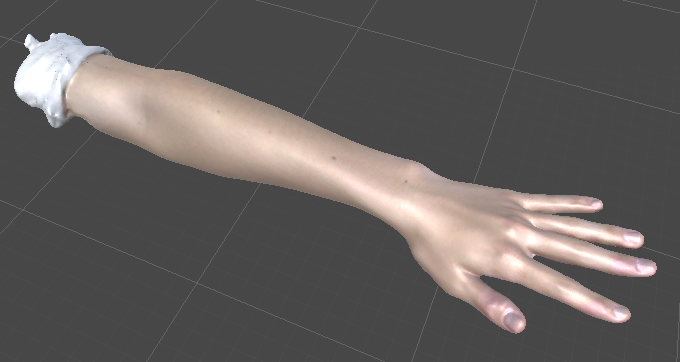
\includegraphics[width = \columnwidth]{../figs/NomalShader.png}
			\end{minipage}
			\hspace{0.04\columnwidth}
			\begin{minipage}{0.4\columnwidth}
			\centering
			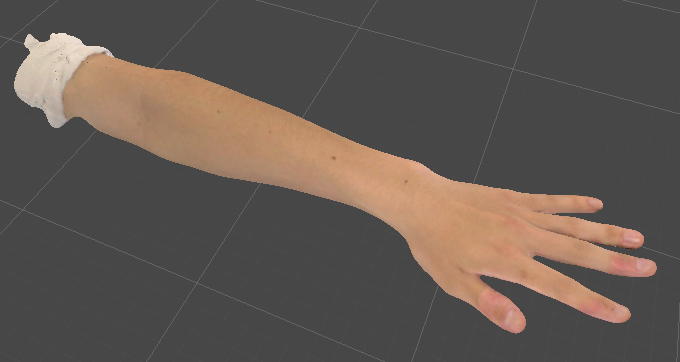
\includegraphics[width = \columnwidth]{../figs/ReflexShader.png}
			\end{minipage}
			\caption{シェーダーによる3Dモデルの違い}
			\end{figure}

		\subsection{オブジェクト}
		\subsection{衝突判定}
			
			\subsubsection{Collider}
			\subsubsection{RayCast}
		\subsection{ペアレント}
		\subsection{ビルド}
			本項ではUnityで構成したシミュレータのビルド方法について解説する。
			以下にビルドの手順を示す。
			\begin{enumerate}
				\item Unityエディタ上のツールバーから"File"を選択
				\item ``Build Settings''の項目を選択すると、別ウィンドウにBuild Settingsが開かれる
				\item 追加したいシーンファイルをUnityエディタ上で開いておき、Build Settingsのウィンドウから"Add Open Scenes"を選択
				\item Build Settings ウィンドウの左にあるPlatformから実行したいOSを選択し、ウィンドウ右下の"Switch Platform"を選択
				\item Build Settings ウィンドウ右下の"build"を選択してビルド開始
			\end{enumerate}
			以上の手順でUnityで作成したシーンのビルドが完了する。
			Windows,LinuxなどのOSではビルドしたフォルダに実行ファイルが作成されているため、
			そのファイルからシミュレータを実行することができる。
			iOS,Android OSに関してはビルド・実行方法が異なるため、それぞれ以下に解説する。
			\subsubsection{iOS}
				本項では、iOS用アプリの実行手順を以下に示す。
				\begin{enumerate}
					\item ビルドされたフォルダをMacOSに転送
					\item MacOSでビルドされたフォルダを開き、フォルダ内の``Unity-iPhone.xcodeproj''をXcodeで開く
					\item iOS端末を接続し、端末の設定から端末をデバッグモードにする
					\item Xcodeウィンドウ上部のAny iOS Device を選択し、接続した端末を選択
					\item Signing&Capabilitiesを選択し、Teamの欄にApple IDを入力
					\item 本シミュレータではBluetoothを用いるため、infoを選択し、Keyの一覧に``Privacy - Bluetooth Peripheral Usage Description''を追加
						し、Valueを``Uses BLE to communicate with devices.''にする
					\item iPhoneにアプリがインストールされたら、端末の『設定』から『プライバシーとセキュリティ』を開き『Bluetooth』を選択
					\item インストールしたアプリにBluetoothの権限を許可する
					\item アプリ一覧からインストールしたアプリを実行する
				\end{enumerate}
				以上の手順でiOS用のシミュレータをビルドして実行できる。
				この手順で一番重要なのが、6の手順でこれがなければアプリを実行してもMade by Unityのポップがでた
				直後に動かなくなってしまう。これらのエラーはXcode上でログが残されているため、発生しているエラーを
				解消すれば実行することができる。大抵の場合、端末側の権限付与ができておらずアプリが実行できないエラーが多発するため
				よく確認をすること。
			\subsubsection{Android OS}
	\section{FirstVR}
		\subsection{デバイス構成}
		\subsection{トラッキング}
		\subsection{キャリブレーション}
	
\chapter{研究手順}
	\section{使用器具}
		本研究での使用器具を表\refeq{tab:usedev}に示す。
	\begin{table}[H]
	\begin{center}
	\caption{本研究における使用器具}
	\label{tab:usedev}
	\begin{tabular}{clllll} \toprule
	No&\multicolumn{1}{l}{機器名}&\multicolumn{1}{l}{型番}&\multicolumn{1}{l}{シリアルNo}&\multicolumn{1}{l}{備考}\\ \hline
	1&EinScan HX&&&\\
	2&FirstVR&UHL-01&&\\
	3&iPhone SE2&&&iOS16.7.2\\
	4&HUAWEI Nova Lite2&&&AndroidOS 9\\
	5&PC-1&&&Ubuntu22.04\\
	6&PC-2&&&MacOS\\
	\bottomrule
	\end{tabular}
	\end{center}
	\end{table}
	以下に本研究で使用したソフトウェアを表\refeq{tab:usesoft}に示す。
	\begin{table}[H]
	\begin{center}
	\caption{使用ソフトウェア}
	\label{tab:usesoft}
	\begin{tabular}{clllll} \toprule
	No&\multicolumn{1}{l}{ソフトウェア名}&\multicolumn{1}{l}{バージョン}&\multicolumn{1}{l}{使用OS}&\multicolumn{1}{l}{備考}\\ \hline
	1&Blender&3.0.1&Ubuntu&\\
	2&Unity&2022.3.11f1&Ubuntu&\\
	3&Xcode&15.0.1&MacOS&\\
	\bottomrule
	\end{tabular}
	\end{center}
	\end{table}
	\section{3Dスキャナ}
		\subsection{3Dモデルの取り込み}
			ハンディ3DスキャナであるEinScan HXを用いて左腕をスキャンした
			本研究では,VHにテクスチャを貼って用いることを前提としているため,
			スキャン形式をRapidスキャンモードで,3Dモデルの精度を高めるために頂点数を
			50万点で出力し,出力形式としてテクスチャがメッシュに割当されている
			obj形式を選択した。
	\section{Blender}
		\subsection{スムージング処理}
			.obj形式で取り込んだ3Dモデルは測定によるノイズが含まれており、特に掌と手の甲の境界線上に
			が段差のように途切れてしまう。このノイズを除去・補完するために、オブジェクト表面の凹凸を
			平坦にする効果があるスムージング処理を行った。
			\begin{figure}[H]
			\centering
			\begin{minipage}{0.4\columnwidth}
			\centering
			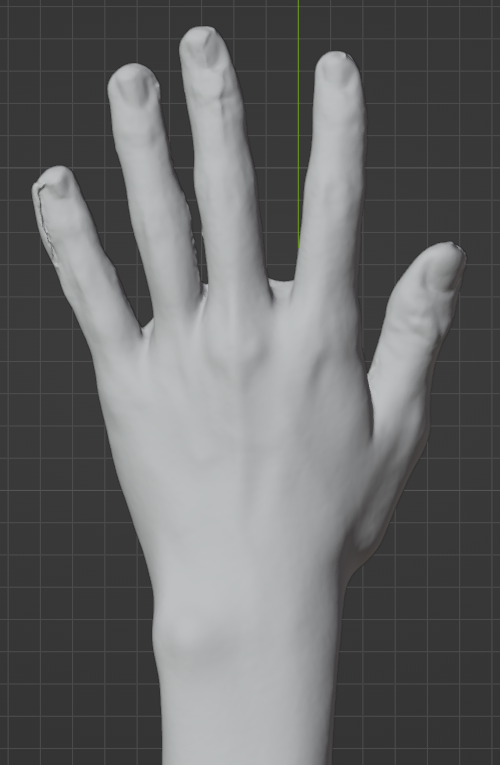
\includegraphics[width = \columnwidth]{../figs/SmoothingBeforRear.png}
			\end{minipage}
			\begin{minipage}{0.4\columnwidth}
			\centering
			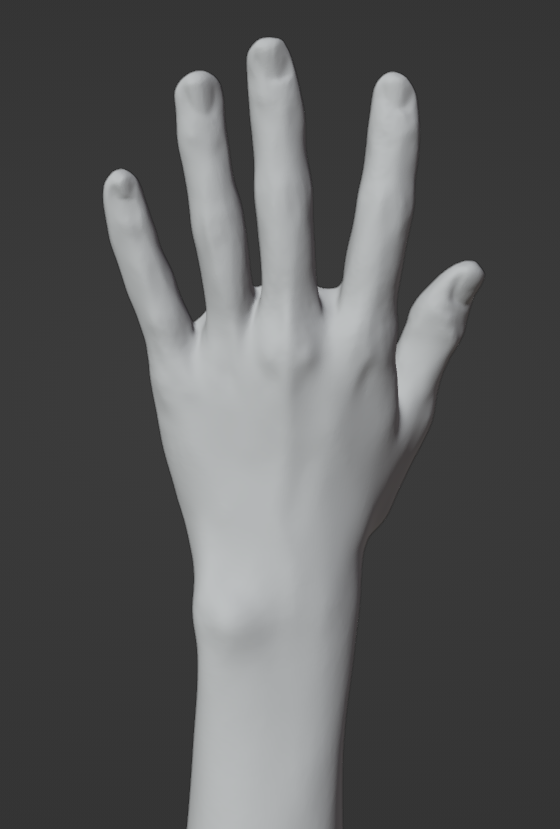
\includegraphics[width = \columnwidth]{../figs/SmoothingAfterRear.png}
			\end{minipage}
			\caption{スムージング処理比較}
			\end{figure}

		\subsection{ボーン配置}
			スムージング処理後の3Dモデルを基準に図のようにボーンを配置した.
			\begin{figure}[H]
			\centering
			\begin{minipage}{0.3\columnwidth}
			\centering
			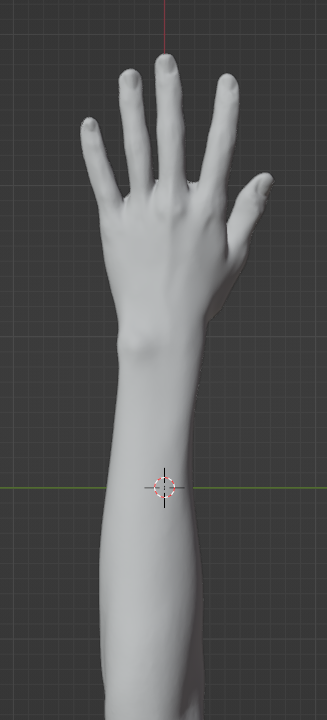
\includegraphics[width = \columnwidth]{../figs/handmeshLat.png}
			\end{minipage}
			\begin{minipage}{0.3\columnwidth}
			\centering
			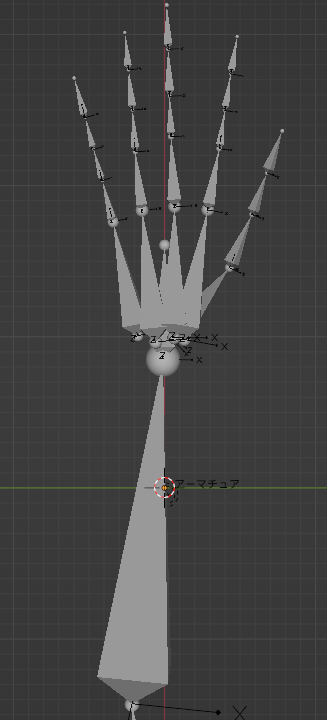
\includegraphics[width = \columnwidth]{../figs/handboneLat.png}
			\end{minipage}
			\caption{ボーン配置図}
			\end{figure}

	\section{Unity}
		\subsection{オブジェクトの処理}
		\subsection{ステージ構成}
		\subsection{アニメーション設定}
			\subsubsection{アニメーションクリップ作成}
			\subsubsection{アニメーター設定}
		\subsection{オブジェクト保持}

		

	\section{FirstVR}
		本研究で構成するシミュレータの入力感度を検証するため、以下の手順でFirstVRの評価を行った。
			\begin{enumerate}
				\item 肘から手首までの長さを測定し、肘を原点に1/4の距離(約7cm)で装着 \\
				\item 端末とFirstVRを接続し、ジェスチャをしていない状態とジェスチャしている状態を学習 \\
				\item ジェスチャをしていない状態の筋変位センサの値を1回測定し,手を握るジェスチャのセンサ値の変化量を5回測定した。
					また,この操作をsample数を7,10〜100までの11段階で測定した。 \\
				\item ノイズの少なかったsample数を選出し、ジェスチャ状態で手の角度を上下左右に動かした場合のノイズを測定 \\
				\item ジェスチャをしていない状態の筋変位センサの値を基準値としてジェスチャ後の測定値との差をとり,各チャネルでの変位量の総和を
					総変化量としてsample数ごとに比較し,最適(分散が少なく,データ量が小さい)なデータを検討した.
			\end{enumerate}
	\section{ビルド}
	\section{評価}

\chapter{研究結果}
	\section{FirstVR}
		\begin{table}[H]
		\begin{center}
		\caption{}
		\label{}
		\begin{tabular}{c|ccccccccccc} \toprule
			num/sample & 7 & 10 & 20 & 30 & 40 & 50 & 60 & 70 & 80 & 90 & 100 \\ \hline
			1 & 44.4 & 25.6 & 21.8 & 19.4 & 12.2 & 12.6 & 13.4 & 22.4 & 8.2 & 11.8 & 27.2 \\
			2 & 37.0 & 23.4 & 30.2 & 17.2 & 27.2 & 31.8 & 45.4 & 26.2 & 29.4 & 19.2 & 18.2 \\
			3 & 23.4 & 20.2 & 28.4 & 20.6 & 21.8 & 30.4 & 17.2 & 23.6 & 39.0 & 17.4 & 22.0 \\
			4 & 49.0 & 69.8 & 108.8 & 100.6 & 78.0 & 62.2 & 61.4 & 40.8 & 60.6 & 36.6 & 37.6 \\
			5 & 38.2 & 53.2 & 51.2 & 34.6 & 35.4 & 43.6 & 46.6 & 48.2 & 47.4 & 32.0 & 37.6 \\
			6 & 31.8 & 15.6 & 17.6 & 38.4 & 23.2 & 23.4 & 32.0 & 37.8 & 14.8 & 22.4 & 22.0 \\
			7 & 69.2 & 44.8 & 57.0 & 25.8 & 33.2 & 39.6 & 23.0 & 33.6 & 53.8 & 29.8 & 40.0 \\
			8 & 67.0 & 66.0 & 55.4 & 65.0 & 67.0 & 78.6 & 93.6 & 59.0 & 66.8 & 59.4 & 65.4 \\
			9 & 44.4 & 25.6 & 21.8 & 19.4 & 12.2 & 12.6 & 13.4 & 22.4 & 8.2 & 11.8 & 27.2 \\
			10 & 20.8 & 13.8 & 15.4 & 16.4 & 13.2 & 17.8 & 43.8 & 17.6 & 12.0 & 83.6 & 14.4 \\
			11 & 24.8 & 22.8 & 26.2 & 21.0 & 27.8 & 48.8 & 41.2 & 15.6 & 23.2 & 14.2 & 19.4 \\
			12 & 34.2 & 29.8 & 19.8 & 25.8 & 24.0 & 18.2 & 32.4 & 25.4 & 35.4 & 35.6 & 25.2 \\
			14 & 20.6 & 17.4 & 21.6 & 29.0 & 19.0 & 22.8 & 27.6 & 32.2 & 56.8 & 44.0 & 31.2 \\
			16 & 19.8 & 22.0 & 11.6 & 10.0 & 16.8 & 17.4 & 12.4 & 17.6 & 21.6 & 15.8 & 11.4 \\
			17 & 50.8 & 58.4 & 51.2 & 56.6 & 67.4 & 37.6 & 45.8 & 52.4 & 51.6 & 59.6 & 56.2 \\
			18 & 35.2 & 50.2 & 62.6 & 36.4 & 27.2 & 39.6 & 38.8 & 43.4 & 45.4 & 52.4 & 48.8 \\
			19 & 49.4 & 42.2 & 41.2 & 36.4 & 49.4 & 34.4 & 33.2 & 34.4 & 22.2 & 13.8 & 36.0 \\
			20 & 23.8 & 26.8 & 36.2 & 38.0 & 28.0 & 35.2 & 34.0 & 24.4 & 29.2 & 39.6 & 25.8 \\
			21 & 33.6 & 11.8 & 10.4 & 16.8 & 17.8 & 11.0 & 19.4 & 13.6 & 24.4 & 13.2 & 9.6 \\
			23 & 32.6 & 36.4 & 33.0 & 17.6 & 22.6 & 26.8 & 32.2 & 25.2 & 20.8 & 30.4 & 13.8 \\
			24 & 32.8 & 42.6 & 36.6 & 30.6 & 26.4 & 41.4 & 32.6 & 20.2 & 25.0 & 15.8 & 17.6 \\
			25 & 42.2 & 27.6 & 37.8 & 33.8 & 39.2 & 50.0 & 34.6 & 38.0 & 38.8 & 26.8 & 24.2 \\
			26 & 51.8 & 40.4 & 44.0 & 44.6 & 41.4 & 39.2 & 42.8 & 38.4 & 41.6 & 43.0 & 30.0 \\
			27 & 38.0 & 30.6 & 38.2 & 35.6 & 23.8 & 20.4 & 24.4 & 24.2 & 22.6 & 30.6 & 16.8 \\
			28 & 25.2 & 33.0 & 32.0 & 23.8 & 28.0 & 20.0 & 31.4 & 13.6 & 19.6 & 19.4 & 21.2 \\
			32 & 39.8 & 32.8 & 30.2 & 38.2 & 34.8 & 22.6 & 30.4 & 24.0 & 24.0 & 12.6 & 20.6 \\
			34 & 68.8 & 78.0 & 50.4 & 51.6 & 44.2 & 50.8 & 40.0 & 48.2 & 46.4 & 48.8 & 62.0 \\
			35 & 20.4 & 29.8 & 40.6 & 45.0 & 23.8 & 25.2 & 27.4 & 39.0 & 25.2 & 28.8 & 39.6 \\
			36 & 32.6 & 29.8 & 21.6 & 19.0 & 22.4 & 17.6 & 21.2 & 28.2 & 41.4 & 35.6 & 20.8 \\
			38 & 23.2 & 8.0 & 13.6 & 23.2 & 21.2 & 25.4 & 24.0 & 12.6 & 16.0 & 24.4 & 17.8 \\
			41 & 44.4 & 25.6 & 21.8 & 19.4 & 12.2 & 12.6 & 13.4 & 22.4 & 8.2 & 11.8 & 27.2 \\
			\bottomrule
		\end{tabular}
		\end{center}
		\end{table}
	\section{シミュレータの定性評価}
\chapter{まとめ}

\chapter{今後の課題}
	現段階では、シミュレータとして最低限の要素を追加した。
	しかし、FirstVRにおける掴みジェスチャの認識精度の低さから本研究で検討しようとした
	リアリティについて検討できなかった。
\clearpage

\chapter*{謝辞}

\begin{thebibliography}{99}

	\bibitem{ref:1}
	芝軒 太郎 他.``VRを利用した筋電義手操作トレーニング
	システムの開発と仮想 Box and Block Test の実現''.
	JRSJ. 2012 July.

	\bibitem{ref:2}
	Osumi M, et al.
	``Characteristics of Phantom Limb Pain Alleviated
	with Virtual Reality Rehabilitation''.
	Pain Med. 2019 May.

	\bibitem{ref:3}
	H2L.Inc.,Tokyo106-0032,Japan;satoshi.hosono@h2l.jp

	\bibitem{ref:4}
	Tamon Miyake, etal``Gait Phase Detection Based on Muscle Deformation
	with Static Standing-Based Calibration''.
	MDPI. 2021 Feb

	\bibitem{ref:5}
	mediVR.Inc.,https://www.medivr.jp/

	\bibitem{ref:6}
	株式会社サンステラ, https://www.einscan.jp/einscan-hx

	\bibitem{ref:7}


\end{thebibliography}
\chapter*{付録}
%ページ番号をローマ数字で表示
\pagenumbering{roman}
%このページから1枚目にカウントしなおす
\setcounter{page}{1}


\end{document}